\documentclass[journal=jacsat,manuscript=article]{achemso}
\usepackage[version=3]{mhchem}
\usepackage{amsmath}
\newcommand*\mycommand[1]{\texttt{\emph{#1}}}
\author{Ana K. Pitol}
\affiliation{Department of Civil and Environmental Engineering, Imperial College
London, United Kingdom}
\email{a.pitol-garcia@imperial.ac.uk}
\author{Timothy R. Julian}
\affiliation{Department of Environmental Microbiology, Eawag, Dubendorf, Switzerland}
\alsoaffiliation{Department of Epidemiology and Public Health, Swiss Tropical and Public
Health Institute, Basel, Switzerland}
\email{tim.julian@eawag.ch}

\abbreviations{IR,NMR,UV}

\keywords{American Chemical Society, \LaTeX}

\title[An \textsf{achemso} demo]{Risk reduction of SARS-CoV-2 transmission through disinfection of
frequently touched surfaces. A Quantitative Microbial Risk Assessment.}
\makeatletter
\ifxetex
  \usepackage[setpagesize=false, % page size defined by xetex
              unicode=false, % unicode breaks when used with xetex
              xetex]{hyperref}
\else
  \usepackage[unicode=true]{hyperref}
\fi
\hypersetup{breaklinks=true,
            bookmarks=true,
            pdfauthor={},
            pdftitle={},
            colorlinks=true,
            urlcolor=blue,
            linkcolor=magenta,
            pdfborder={0 0 0}}
\urlstyle{same}  % don't use monospace font for urls
% pandoc header

\begin{document}
\begin{abstract}
not exceeding 200 words A graphic for the Table of Contents (TOC) must
be supplied with each Letter This graphic can be no wider than 8 cm and
no taller than 4 cm and should be prepared following the specifications
under Artwork.
\end{abstract}
\begin{tocentry}
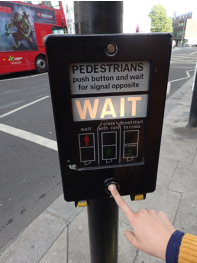
\includegraphics{Risk-reduction-of-SARS-CoV-2-by-disinfection-of-surfaces-and-hands_files/figure-latex/TOC.pdf}
\end{tocentry}

\hypertarget{introduction}{%
\section{Introduction}\label{introduction}}

SARS-CoV-2, the virus responsible for the COVID-19 pandemic, is
transmitted via both direct (person-to-person) and indirect (via a
contaminated environment) routes.\textsuperscript{1,2} Direct
transmission appears to be the leading route and occurs via prolonged
exposures to respiratory droplets produced while talking, coughing, and
sneezing. Infection control recommendations, based on the assumption
that direct contact transmission is the leading route, include
maintaining social/physical distances, wearing masks, case isolation,
contact tracing, and quarantine.\textsuperscript{3}

Despite knowledge that SARS-CoV-2 transmission is primarily through
direct transmission, indirect transmission - or transmission occurring
due to interaction with a contaminated environment -- remains possible.
People infected with SARS-CoV-2 shed the virus into the environment, as
evidenced by extensive environmental contamination detected on surfaces
in cruise ships, hospitals, and public spaces in urban areas such as bus
stations and public squares {[}4; 5; Abrahao2020{]}. Infective
coronavirus persists in the environment, with experimental evidence of
persistence on surfaces for prolonged periods up to 9
days.\textsuperscript{6} Viruses readily transfer from contaminated
surfaces to the skin upon contact\textsuperscript{7--11} and from the
skin to the mouth and saliva of individuals.\textsuperscript{10,12}
Taken together, this evidence suggests surface contamination poses a
risk for indirect SARS-CoV-2 transmission, similar to other respiratory
viruses.\textsuperscript{13}

Indirect transmission events of SARS-CoV-2, even if not the dominant
transmission route, complicate infection control efforts using contact
tracing. Contact tracing efforts focus on identifying people sharing
spaces coincidentally with cases.\textsuperscript{3} Indirect
transmission could occur in the absence of shared spaces. As an example,
transmission of SARS-CoV-1 in a Taiwanese hospital led to nosocomial
infection of 31 patients. In 6 (20\%) of the patients, contact tracing
failed to detect direct contacts with other SARS patients, although RNA
of SARS-CoV-1 was detected throughout the hospital on drinking water
buttons, beds, and chairs.\textsuperscript{14} Based on these findings,
the authors suggest indirect transmission as the cause of transmission
amongst a subset of those infected.\textsuperscript{14} If indirect
transmission is an important route for SARS-CoV-2, control strategies
will necessarily have to integrate hand hygiene interventions and
surface disinfection alongside contact tracing.\textsuperscript{15}

Despite the potential importance of indirect transmission, it is
difficult to estimate its importance relative to direct
transmission.\textsuperscript{16} Quantitative Microbial Risk Analysis
(QMRA) provides a framework for understanding health risks from indirect
transmission and provides insights into potential impacts of infection
control recommendations. Mechanistic models of fomite-mediated
transmission events within the context of QMRA frameworks have been used
to inform risks for children interacting with contaminated
toys,\textsuperscript{17} sanitation workers collecting and processing
urine for nutrient recovery,\textsuperscript{18} transmission of
norovirus within a houseboat,\textsuperscript{19} and impact of surface
disinfection.\textsuperscript{20} QMRA has also been adapted to evaluate
risks for hospital transmission of MERS-CoV through droplets and
aerosolized particles. The analysis highlighted reductions in risk to
hospital staff through mask use (\textgreater90\% estimated risk
reduction) and increased air exchange (up to 58\% estimated risk
reduction).\textsuperscript{21}

\textbf{???} QMRA to evaluate the reduction in the risk of infection of
SARS-CoV-2 for mask wearers.

In this study, a mechanistic model of indirect transmission within the
QMRA framework is developed to estimate likelihood of transmission in
community settings and inform guidance on surface disinfection
strategies. Specifically, the risks of infection with SARS-CoV-2 are
estimated for interactions with shared spaces (i.e., use of ATMs,
buttons on cross walks and trains). Risk reductions are further
estimated under various feasible surface disinfection strategies.

\hypertarget{materials-and-methods}{%
\section{Materials and Methods}\label{materials-and-methods}}

We modeled the risk of SARS-CoV-2 infection due to contact with
frequently touched buttons and estimated the effect that different
surface disinfection practices have on infection risk. The sequence of
events leading to the viral inoculation of the susceptible individual is
considered to be the following: 1) contamination event (infected person
coughing on the hand followed by a hand-to-surface contact), 2) virus
decay on the surface, 3) virus transfer from the surface to finger, and
4) virus transfer from finger to facial mucous membranes. The
stochastic-mechanistic model used herein is based on models described
elsewhere.\textsuperscript{17,22} Two scenarios were considered: risk of
infection with and without surface disinfection. Additionally, different
disinfection regimes were tested.

Viral loads in the saliva or sputum of symptomatic COVID-19 patients
within the first 14 days of symptom onset were used as model input. The
viral loads were measured using quantitative reverse-transcription
polymerase chain reaction (RT-qPCR).\textsuperscript{23--26} PCR data
does not distinguish between infectious and non-infectious virus. To
convert gene copies to infections virus, we used a ratio reported for
influenza viruses.\textsuperscript{27}

The proportion of viral particles emitted in a cough that is transferred
to the hand when the hand is used to cover the mouth was estimated using
a conical dispersion model\textsuperscript{28} - the particles were
assumed to be conically spread over a 80 angle, at a distance of 5cm.
The transfer of viruses from the hand of the infected individual to the
surface was estimated with: \(Csurface=Chand*TEsh\), where \(Chand\) is
the concentration of viruses on the hand \([virus/cm^2]\), and TEsh
\([%]
\) is the transfer efficiency of viruses between the surface (assumed to
be metal) and the hand. Once the surface was contaminated, the
concentration of virus in the surface at any given time was calculated
as follows \(Csurf(t)= Csurf(0)\) \(e^{-nt}\), where \(Csurf(t)\)
\([virus/cm^2]\) is the concentration of infective viruses at time
\(t\), \(Csurf(0)\) \([virus/cm2^]\) is the initial concentration of
virus in the surface, \(t\) \([min]\) is the time lapsed after surface
inoculation, and \(n\) \([m^{-1}]\) is the decay rate of the virus in
the selected surface (metal or plastic).

\hypertarget{alternative-way-of-presenting-the-equations}{%
\subsection{Alternative way of presenting the
equations}\label{alternative-way-of-presenting-the-equations}}

The equations can be presented as follows:

(Eq. \ref{eqn:Inactivation}) \begin{equation}
C(t)= C(0) e^{-nt} \label{eqn:Inactivation}
\end{equation}

(Eq. \ref{eqn:Transfer_sh}) \begin{equation}
C_{f_f} = C(t) TE_{sh} \label{eqn:Transfer_sh}
\end{equation}

(Eq. \ref{eqn:Dose}) \begin{equation}
D = C_{h} S_{hm} TE_{hm} \label{eqn:Dose}
\end{equation}

(Eq. \ref{eqn:DoseResponse}) \begin{equation}
P_{inf}=1 - e^{-kD} \label{eqn:DoseResponse}
\end{equation}

\hypertarget{results-and-discussion}{%
\section{Results and discussion}\label{results-and-discussion}}

Frequently touched surfaces such as and train buttons and traffic light
buttons are of risk concern due to their frequent use by multiple
people. SARS-CoV-2 contamination has been reported in public surfaces of
an urban area in Brazil. The concentration of viruses was between 20 and
2990 genome units per m\(^2\). The surfaces were bench, ground, handrail
made out metal, and concrete.\textsuperscript{29} In this article, we
estimated the risk of contacting frequently touched surfaces as a
function of the prevalence of infection within the population and
evaluated the reduction of risk based on different disinfection methods.

`` How big the droplets need to be and how far away they can travel is
still an open question"

\hypertarget{floats}{%
\subsection{Floats}\label{floats}}

New float types are automatically set up by the class file. The means
graphics are included as follows (Scheme \ref{sch:example}). As
illustrated, the float is ``here'' if possible.

\begin{scheme}
  Your scheme graphic would go here: \texttt{.eps} format\\
  for \LaTeX\, or \texttt{.pdf} (or \texttt{.png}) for pdf\LaTeX\\
  \textsc{ChemDraw} files are best saved as \texttt{.eps} files:\\
  these can be scaled without loss of quality, and can be\\
  converted to \texttt{.pdf} files easily using \texttt{eps2pdf}.\\
  %\includegraphics{graphic}
  \caption{An example scheme}
  \label{sch:example}
\end{scheme}

\begin{figure}
\centering
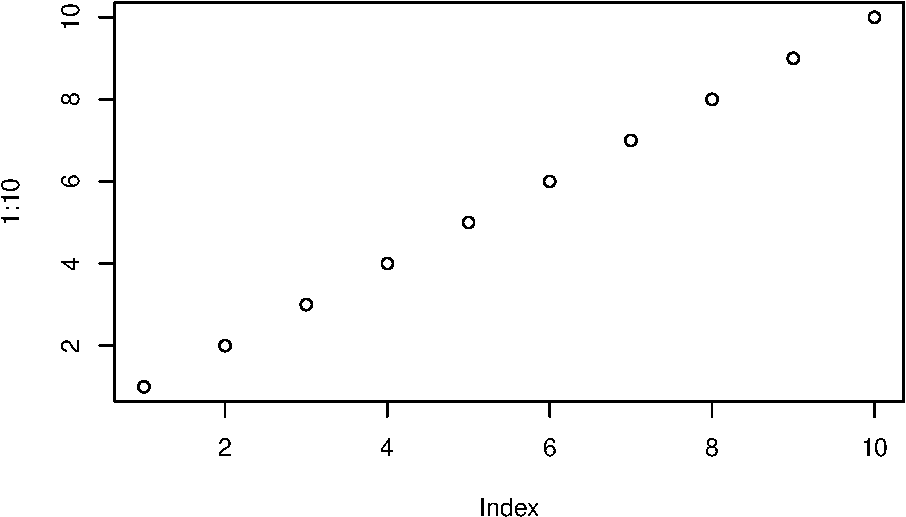
\includegraphics{Risk-reduction-of-SARS-CoV-2-by-disinfection-of-surfaces-and-hands_files/figure-latex/unnamed-chunk-1-1.pdf}
\caption{test}
\end{figure}

\begin{figure}
  As well as the standard float types \texttt{table}\\
  and \texttt{figure}, the class also recognises\\
  \texttt{scheme}, \texttt{chart} and \texttt{graph}.
  \caption{An example figure}
  \label{fgr:example}
\end{figure}

Charts, figures and schemes do not necessarily have to be labelled or
captioned. However, tables should always have a title. It is possible to
include a number and label for a graphic without any title, using an
empty argument to the \texttt{\textbackslash caption} macro.

The use of the different floating environments is not required, but it
is intended to make document preparation easier for authors. In general,
you should place your graphics where they make logical sense; the
production process will move them if needed.

\begin{acknowledgement}
The author thanks Sunil Dogga, Emmanuel Frousteyand, and Danilo Cuccato for their help with the model. 
\end{acknowledgement}

\begin{suppinfo}
Experimental procedures and
characterization data for all new compounds. The class will
automatically add a sentence pointing to the information on-line:
\end{suppinfo}

\hypertarget{references}{%
\subsection*{References}\label{references}}
\addcontentsline{toc}{subsection}{References}

\hypertarget{refs}{}
\leavevmode\hypertarget{ref-WHO2020}{}%
(1) WHO. \emph{Scientific brief} \textbf{2020}, \emph{29} (March),
10--12.

\leavevmode\hypertarget{ref-CDC2020}{}%
(2) CDC. \emph{How COVID-19 Spreads}; 2020; Vol. 2019, p 2020.

\leavevmode\hypertarget{ref-Ferretti2020}{}%
(3) Ferretti, L.; Wymant, C.; Kendall, M.; Zhao, L.; Nurtay, A.;
Abeler-Dörner, L.; Parker, M.; Bonsall, D.; Fraser, C. \emph{Science}
\textbf{2020}, \emph{368} (6491), 0--8.

\leavevmode\hypertarget{ref-Ong2020}{}%
(4) Ong, S. W. X.; Tan, Y. K.; Chia, P. Y.; Lee, T. H.; Ng, O. T.; Wong,
M. S. Y.; Marimuthu, K. \emph{JAMA - Journal of the American Medical
Association} \textbf{2020}, 2--4.

\leavevmode\hypertarget{ref-Ye2020}{}%
(5) Ye, G.; Lin, H.; Chen, L.; Wang, S.; Zeng, Z.; Wang, W.; Zhang, S.;
Rebmann, T.; Li, Y.; Pan, Z.; Yang, Z.; Wang, Y.; Wang, F.; Qian, Z.;
Wan, X. \emph{medRxiv preprint} \textbf{2020}, 1--20.

\leavevmode\hypertarget{ref-Kampf2020}{}%
(6) Kampf, G.; Todt, D.; Pfaender, S.; Steinmann, E. \emph{Journal of
Hospital Infection} \textbf{2020}, \emph{104} (3), 246--251.

\leavevmode\hypertarget{ref-Julian2010}{}%
(7) Julian, T. R.; Leckie, J. O.; Boehm, A. B. \emph{Journal of Applied
Microbiology} \textbf{2010}, \emph{109}, 1868--1874.

\leavevmode\hypertarget{ref-Lopez2013}{}%
(8) Lopez, G. U.; Gerba, C. P.; Tamimi, A. H.; Kitajima, M.; Maxwell, S.
L.; Rose, J. B. \emph{Applied and Environmental Microbiology}
\textbf{2013}, \emph{79}, 5728--5734.

\leavevmode\hypertarget{ref-Bidawid2004}{}%
(9) Bidawid, S.; Malik, N.; Adegbunrin, O.; Sattar, S. A.; Farber, J. M.
\emph{J Food Prot} \textbf{2004}, \emph{67} (1), 103--109.

\leavevmode\hypertarget{ref-Rusin2002}{}%
(10) Rusin, P.; Maxwell, S.; Gerba, C. \emph{Journal of Applied
Microbiology} \textbf{2002}, \emph{93}, 585--592.

\leavevmode\hypertarget{ref-Ansari1991}{}%
(11) Ansari, S.; Springthorpe, V.; Sattar, S.; Rivard, S.; Rahman, M.
\emph{Journal of Clinical Microbiology} \textbf{1991}, \emph{29} (10),
2115--2119.

\leavevmode\hypertarget{ref-Pitol2017}{}%
(12) Pitol, A. K.; Bischel, H. N.; Kohn, T.; Julian, T. R.
\emph{Environmental Science and Technology} \textbf{2017}.

\leavevmode\hypertarget{ref-Boone2007}{}%
(13) Boone, S. A.; Gerba, C. P. \emph{Applied and Environmental
Microbiology} \textbf{2007}, \emph{73} (6), 1687--1696.

\leavevmode\hypertarget{ref-Chen2004}{}%
(14) Chen, Y. C.; Huang, L. M.; Chan, C. C.; Su, C. P.; Chang, S. C.;
Chang, Y. Y.; Chen, M. L.; Hung, C. C.; Chen, W. J.; Lin, F. Y.; Lee, Y.
T.; Chen, D. S.; Lee, Y. T.; Teng, C. M.; Yang, P. C.; Ho, H. N.; Chen,
P. J.; Chang, M. F.; Wang, J. T.; Kao, C. L.; Wang, W. K.; Hsiao, C. H.;
Hsueh, P. R. \emph{Emerging Infectious Diseases} \textbf{2004},
\emph{10} (5), 782--788.

\leavevmode\hypertarget{ref-Mcclellan2020}{}%
(15) Gottlieb, S.; Rivers, C.; Mcclellan, M. B.; Silvis, L.; Watson, C.
\emph{American Enterprise Institute} \textbf{2020}, 1--16.

\leavevmode\hypertarget{ref-BarOn2020}{}%
(16) Bar-on, Y. M.; Flamholz, A.; Phillips, R.; Milo, R. \emph{eLife}
\textbf{2020}.

\leavevmode\hypertarget{ref-Julian2009}{}%
(17) Julian, T. R.; Canales, R. a.; Leckie, J. O.; Boehm, A. B.
\emph{Risk Analysis} \textbf{2009}, \emph{29}, 617--632.

\leavevmode\hypertarget{ref-Bischel2019}{}%
(18) Bischel, H. N.; Caduff, L.; Schindelholz, S.; Kohn, T.; Julian, T.
R. \emph{Environmental Science and Technology} \textbf{2019}, \emph{53}
(12), 7055--7067.

\leavevmode\hypertarget{ref-Canales2019}{}%
(19) Canales, R. A.; Reynolds, K. A.; Wilson, A. M.; Fankem, S. L. M.;
Weir, M. H.; Rose, J. B.; Abd-Elmaksoud, S.; Gerba, C. P. \emph{Journal
of Occupational and Environmental Hygiene} \textbf{2019}, \emph{16} (1),
16--26.

\leavevmode\hypertarget{ref-Ryan2014a}{}%
(20) Ryan, M. O.; Haas, C. N.; Gurian, P. L.; Gerba, C. P.; Panzl, B.
M.; Rose, J. B. \emph{American Journal of Infection Control}
\textbf{2014}, \emph{42} (11), 1165--1172.

\leavevmode\hypertarget{ref-Adhikari2019}{}%
(21) Adhikari, U.; Chabrelie, A.; Weir, M.; Boehnke, K.; McKenzie, E.;
Ikner, L.; Wang, M.; Wang, Q.; Young, K.; Haas, C. N.; Rose, J.;
Mitchell, J. \emph{Risk Analysis} \textbf{2019}, \emph{39} (12),
2608--2624.

\leavevmode\hypertarget{ref-Julian2018}{}%
(22) Julian, T. R.; Vithanage, H. S. K.; Chua, M. L.; Kuroda, M.; Pitol,
A. K.; Nguyen, P. H. L.; Canales, R. A.; Fujii, S.; Harada, H.
\emph{Science of The Total Environment} \textbf{2018}, \emph{635},
120--131.

\leavevmode\hypertarget{ref-Wolfel2020}{}%
(23) Wölfel, R.; Corman, V. M.; Guggemos, W.; Seilmaier, M.; Zange, S.;
Müller, M. A.; Niemeyer, D.; Jones, T. C.; Vollmar, P.; Rothe, C.;
Hoelscher, M.; Bleicker, T.; Brünink, S.; Schneider, J.; Ehmann, R.;
Zwirglmaier, K.; Drosten, C.; Wendtner, C. \emph{Nature} \textbf{2020},
1--14.

\leavevmode\hypertarget{ref-Pan2020}{}%
(24) Pan, Y.; Zhang, D.; Yang, P.; Poon, L. L. M.; Wang, Q. \emph{The
Lancet Infectious Diseases} \textbf{2020}, \emph{20} (4), 411--412.

\leavevmode\hypertarget{ref-Kim2020}{}%
(25) Kim, J. Y.; Ko, J. H.; Kim, Y.; Kim, Y. J.; Kim, J. M.; Chung, Y.
S.; Kim, H. M.; Han, M. G.; Kim, S. Y.; Chin, B. S. \emph{Journal of
Korean Medical Science} \textbf{2020}, \emph{35} (7), 1--7.

\leavevmode\hypertarget{ref-To2020}{}%
(26) To, K. K. W.; Tsang, O. T. Y.; Leung, W. S.; Tam, A. R.; Wu, T. C.;
Lung, D. C.; Yip, C. C. Y.; Cai, J. P.; Chan, J. M. C.; Chik, T. S. H.;
Lau, D. P. L.; Choi, C. Y. C.; Chen, L. L.; Chan, W. M.; Chan, K. H.;
Ip, J. D.; Ng, A. C. K.; Poon, R. W. S.; Luo, C. T.; Cheng, V. C. C.;
Chan, J. F. W.; Hung, I. F. N.; Chen, Z.; Chen, H.; Yuen, K. Y.
\emph{The Lancet Infectious Diseases} \textbf{2020}, \emph{20} (5),
565--574.

\leavevmode\hypertarget{ref-Ip2016}{}%
(27) Ip, D. K. M.; Lau, L. L. H.; Chan, K. H.; Fang, V. J.; Leung, G.
M.; Peiris, M. J. S.; Cowling, B. J. \emph{Clinical Infectious Diseases}
\textbf{2015}, \emph{62} (4), 431--437.

\leavevmode\hypertarget{ref-Nicas2009}{}%
(28) Nicas, M.; Jones, R. M. \emph{Risk Analysis} \textbf{2009},
\emph{29} (9), 1292--1303.

\leavevmode\hypertarget{ref-Abrahao2020}{}%
(29) Abrahao, J. S.; Pengo, L. S.; Rezende, I. M.; Rodrigues, R.;
Crispim, A. P. C.; Moura, C. C.; Mendonca, D. C.; Reis, E.; Souza, F.;
Oliveira, G. F. G. G. P. G.; Domingos, I. J. da S.; Boratto, P.; Silva,
P. H. B. e; Queiroz, V. F.; Silva, T. B. de S.; Oliveira, G. F. G. G. P.
G.; Alves, V. de S.; Alves, P. A.; Kroon, E. G.; Trindade, G. de S.;
Drumond, B. P.; Jônatas, A.; Abrahão, S.; Sacchetto, L.; Rezende, I. M.;
Rodrigues, R.; Paula, A.; Crispim, C.; Moura, C. C.; Correa, D.; Reis,
E.; Souza, F.; Fernanda, G.; Oliveira, G. F. G. G. P. G.; José, I.;
Domingos, S.; Boratto, P.; Henrique, P. \emph{medRxiv} \textbf{2020}.
\end{document}
